\documentclass[11pt,a4paper]{article}
\usepackage[margin=1in]{geometry}
\usepackage{graphicx}
\title{FIGURES1\_5\_SYNTHESIS\_2026-03-08\\Scientific Milestone Report}
\author{Science-Chief}
\date{2026-03-08}
\begin{document}
\maketitle

\section*{1. Scope}
This report interprets the first five ERC8004 figures in one coherent scientific narrative.

\section*{2. Data Origin and Why They Matter}
Data come from Ethereum ERC8004 registries:
Identity Registry \texttt{0x8004A169FB4a3325136EB29fA0ceB6D2e539a432} and Reputation Registry \texttt{0x8004BAa17C55a88189AE136b182e5fdA19dE9b63}.
We extract these events to answer three questions: (i) adoption vs activation, (ii) concentration structure, (iii) semantic usage of feedback tags.

\section*{3. Extraction-to-Analysis Link}
Event logs were decoded into structured CSV files (registered, transfer, newfeedback). Figures 1--5 are deterministic transforms of those tables:
\begin{itemize}
\item Figure 1: cumulative registrations vs feedback events;
\item Figure 2: per-agent top-1 client share distribution;
\item Figure 3: client-side Lorenz concentration curve;
\item Figure 4: time to first feedback distribution;
\item Figure 5: top \texttt{tag1} frequency distribution.
\end{itemize}

\section*{4. Results}
\begin{figure}[htbp]\centering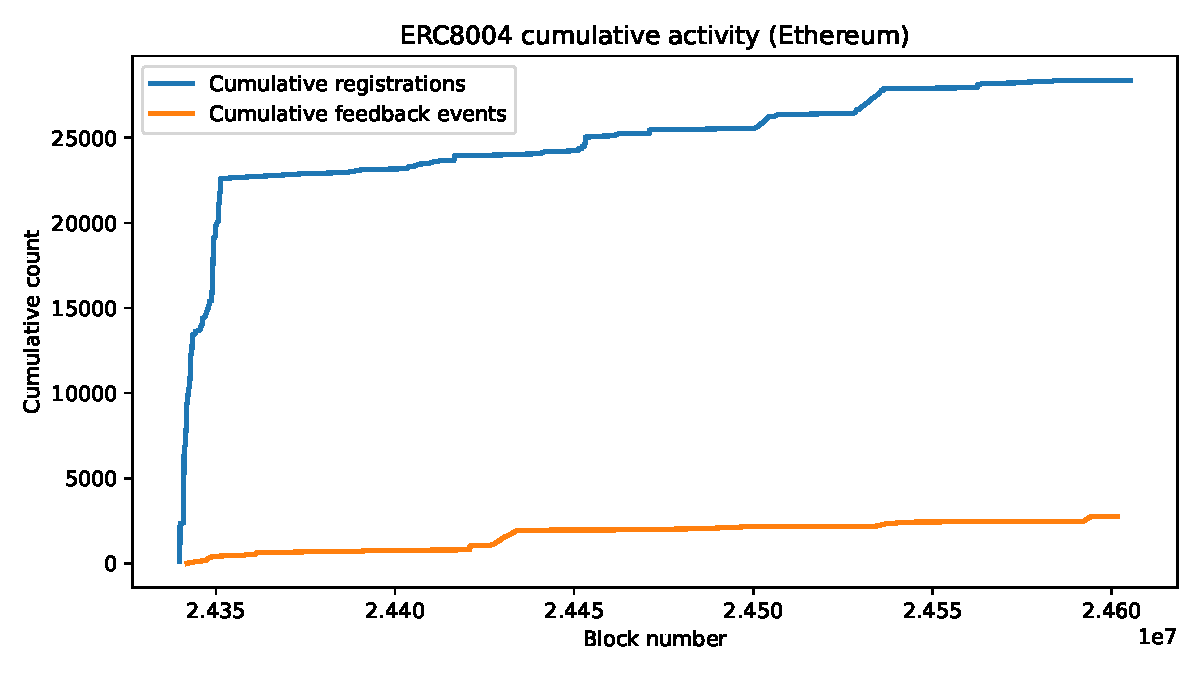
\includegraphics[width=0.86\textwidth]{figures/fig_01_cumulative_activity.pdf}\caption{Figure 1.}\end{figure}
\begin{figure}[htbp]\centering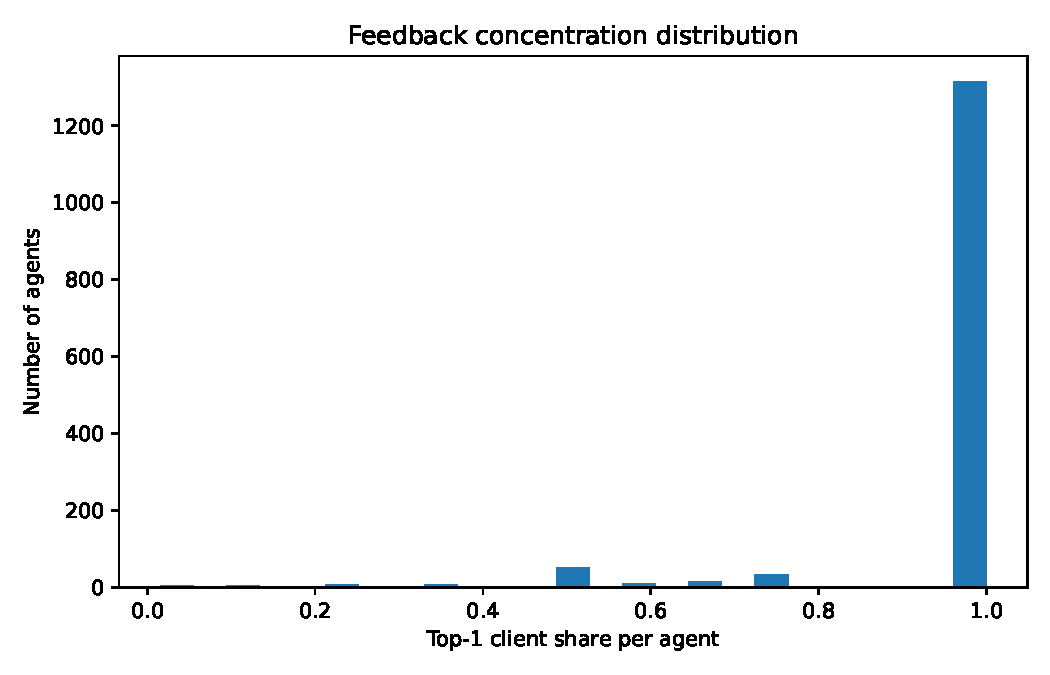
\includegraphics[width=0.86\textwidth]{figures/fig_02_feedback_concentration_hist.pdf}\caption{Figure 2.}\end{figure}
\begin{figure}[htbp]\centering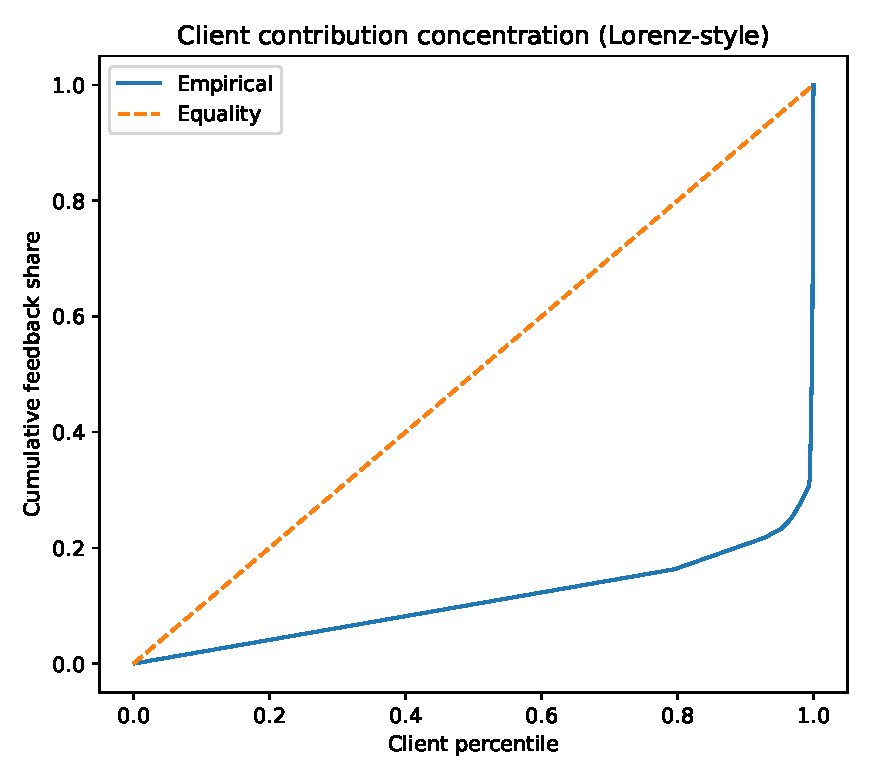
\includegraphics[width=0.86\textwidth]{figures/fig_03_client_concentration_lorenz.pdf}\caption{Figure 3.}\end{figure}
\begin{figure}[htbp]\centering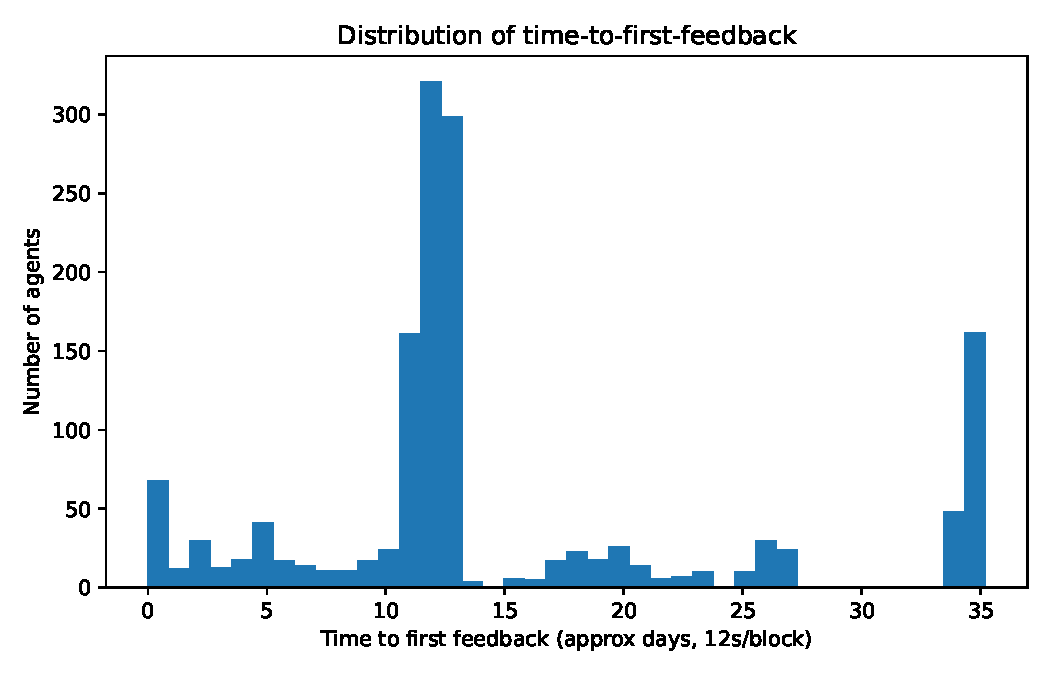
\includegraphics[width=0.86\textwidth]{figures/fig_04_time_to_first_feedback_days.pdf}\caption{Figure 4.}\end{figure}
\begin{figure}[htbp]\centering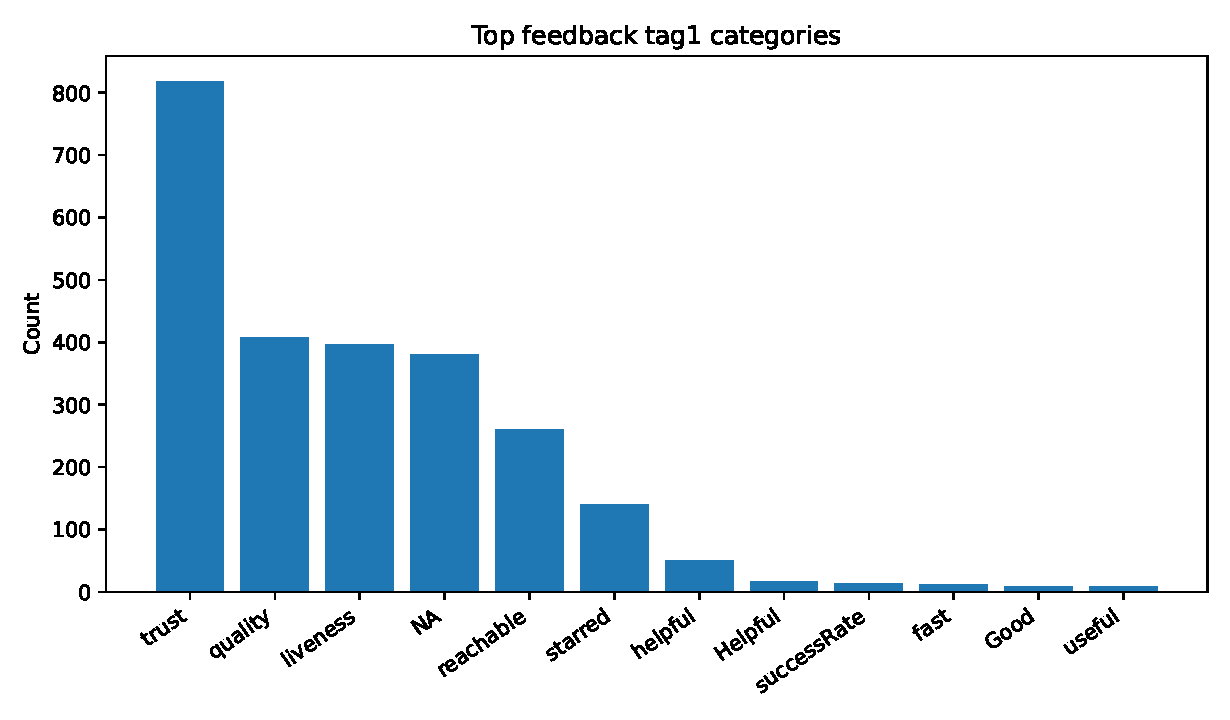
\includegraphics[width=0.86\textwidth]{figures/fig_05_feedback_tag1_top12.pdf}\caption{Figure 5.}\end{figure}

Quantitative context: 28,380 registered agents, 2,776 feedback events, 1,470 agents with feedback (coverage \~5.18\%).

\section*{5. Interpretation (SC)}
The five figures jointly indicate a sparse activation regime: identity growth is broad, but reputation activation is narrow and concentrated. Concentration appears both at the per-agent level (single-client dominance) and global client issuance level. Semantic interpretation of \texttt{tag1} is informative but still sensitive to missing/normalization effects.

\section*{6. Limitations}
ETH-only scope; proxy-time caveat for Figure 4; semantic caveat for Figure 5 (NA and normalization).

\section*{7. Decision and Next Actions}
\textbf{Decision: GO internal, HOLD for strong external semantic claims.}
Next: complete semantic QA, robustness splits, and timestamp-enriched timing panel.

\section*{Appendix: Source Paths}
\textbf{Figures}\\
\begin{itemize}
\item \texttt{workspaces/science-chief/outbox/Reports/FIGURES1\_5\_SYNTHESIS\_2026-03-08/figures/fig\_01\_cumulative\_activity.pdf}
\item \texttt{workspaces/science-chief/outbox/Reports/FIGURES1\_5\_SYNTHESIS\_2026-03-08/figures/fig\_02\_feedback\_concentration\_hist.pdf}
\item \texttt{workspaces/science-chief/outbox/Reports/FIGURES1\_5\_SYNTHESIS\_2026-03-08/figures/fig\_03\_client\_concentration\_lorenz.pdf}
\item \texttt{workspaces/science-chief/outbox/Reports/FIGURES1\_5\_SYNTHESIS\_2026-03-08/figures/fig\_04\_time\_to\_first\_feedback\_days.pdf}
\item \texttt{workspaces/science-chief/outbox/Reports/FIGURES1\_5\_SYNTHESIS\_2026-03-08/figures/fig\_05\_feedback\_tag1\_top12.pdf}
\end{itemize}
\textbf{Tables}\\
\begin{itemize}
\item \texttt{workspaces/science-chief/outbox/Reports/FIGURES1\_5\_SYNTHESIS\_2026-03-08/tables/figures15\_keymetrics\_table.tex}
\end{itemize}

\end{document}
